\documentclass[../../InformazioneQuantistica.tex]{subfiles}

\begin{document}

\section{Quantificare l'informazione}
\lesson{11 \greendot}{3/4/2019}

Ci dedichiamo ora al problema di \textit{quantificare} le correlazioni quantistiche. Per far ciò è necessario innanzitutto definire il problema, cercando un metodo preciso per \textit{quantificare} qualcosa di astratto come \q{l'informazione} contenuta in un messaggio. 

\subsection{Entropia di Shannon}
Partiamo allora introducendo alcuni concetti di teoria dell'informazione \textit{classica}. Il problema di \textit{quantificare} l'informazione contenuta in un messaggio fu risolto da Shannon nel 1948, sfruttando un'analogia  tra la \textit{complessità} di un sistema fisico (che è \q{codificata} dalla sua entropia) e quella di un \textit{sequenza di caratteri}.\\

Partiamo da alcune definizioni di base:
\begin{itemize}
\item Un \textbf{messaggio} è una sequenza di lunghezza arbitraria $N$ composta di \textbf{lettere} scelte da un certo \textbf{alfabeto} $\mathcal{A}$:
\begin{align*}
\mathcal{A} = \{ a_1, \dots, a_k\}
\end{align*}
Assumiamo per semplicità che le lettere nel messaggio siano \textbf{statisticamente indipendenti} l'una dall'altra. Precisamente, ciò significa che ogni lettera compare in una qualsiasi posizione nel messaggio con una probabilità $p_i$ (conosciuta a priori) che non dipende dalle lettere che la precedono o la seguono\footnote{Ciò è chiaramente falso nel caso di messaggi scritti in una \textit{lingua naturale}, come l'italiano. Per esempio è molto difficile che $k$ segua una $m$, ed è molto probabile che una $u$ segua una $q$.}. Naturalmente le $p_i$ devono rispettare le condizioni proprie delle probabilità:
\begin{align*}
p_i \geq 0 \quad \forall i=1,\dots, k; \qquad \sum_{i=1}^k p_i = 1
\end{align*}
\end{itemize}

Consideriamo allora una distribuzione di probabilità fissata, ossia la sequenza delle probabilità delle $k$ lettere dell'alfabeto: $\{p_1, p_2, \dots, p_k\}$. Si definisce \textbf{entropia di Shannon} la quantità:
\begin{align*}
H(p_1, \dots, p_k) = -\sum_{i=1}^k p_i \log_2 p_i
\end{align*}
dove la base del logaritmo è una scelta convenzionale (in genere si usa $2$ con riferimento all'alfabeto binario), e verrà spesso omessa.\\

\textbf{Esempio}. Un messaggio binario ha caratteri scelti da un alfabeto di soli due elementi: $\mathcal{A}=\{0,1\}$. Avremo quindi $0 \leq p_1 \equiv p \leq 1$, e $p_2 = 1-p$, da cui l'entropia di Shannon è data da:
\begin{align}
H(p_1, p_2) = -p \log_2 p - (1-p)\log_2(1-p) = H(p)
\label{eqn:mistura-classica}
\end{align}

\begin{figure}[H]
\centering
\tikzset{every picture/.style={line width=0.75pt}} %set default line width to 0.75pt        

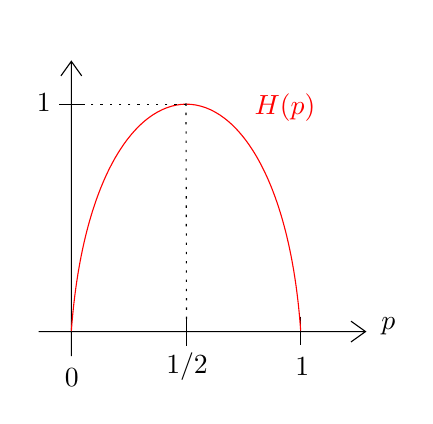
\begin{tikzpicture}[x=0.75pt,y=0.75pt,yscale=-1,xscale=1]
%uncomment if require: \path (0,300); %set diagram left start at 0, and has height of 300

%Shape: Axis 2D [id:dp03836096767914454] 
\draw  (184,209.7) -- (341.5,209.7)(199.75,79.5) -- (199.75,221.5) (334.5,204.7) -- (341.5,209.7) -- (334.5,214.7) (194.75,86.5) -- (199.75,79.5) -- (204.75,86.5)  ;
%Straight Lines [id:da09029121839767407] 
\draw    (310.25,202.5) -- (310.25,216) ;


%Straight Lines [id:da6499966939007862] 
\draw    (206.25,100.4) -- (193.75,100.4) ;


%Curve Lines [id:da6597373551550418] 
\draw [color={rgb, 255:red, 255; green, 0; blue, 0 }  ,draw opacity=1 ]   (199.75,209.5) .. controls (210.4,63.55) and (300,63.88) .. (310.25,209.25) ;


%Straight Lines [id:da4829975793327501] 
\draw    (255.25,203) -- (255.25,216.5) ;


%Straight Lines [id:da4265093472437165] 
\draw  [dash pattern={on 0.84pt off 2.51pt}]  (255,99.8) -- (255.25,204.5) ;


%Straight Lines [id:da9213182147125973] 
\draw  [dash pattern={on 0.84pt off 2.51pt}]  (255,100.2) -- (206.6,100.2) ;



% Text Node
\draw (352.5,207) node   {$p$};
% Text Node
\draw (302.7,101.6) node [color={rgb, 255:red, 255; green, 0; blue, 0 }  ,opacity=1 ]  {$H( p)$};
% Text Node
\draw (200,232) node   {$0$};
% Text Node
\draw (311,226.5) node   {$1$};
% Text Node
\draw (186.5,99.5) node   {$1$};
% Text Node
\draw (255.5,226.5) node   {$1/2$};


\end{tikzpicture}
\caption{Grafico dell'entropia di Shannon $H(p)$ per un messaggio binario.\label{plot:shannon-binario}}
\end{figure}

Notiamo\marginpar{Interpretazione dell'entropia di Shannon} che $H(p)=0$ per $p=0$ o $p=1$. In altre parole messaggi \textit{costanti}, cioè formati da soli $0$ o soli $1$ hanno entropia \textit{minima} (nulla). Viceversa, un messaggio in cui $0$ e $1$ compaiono con la stessa probabilità ha entropia \textit{massima}.\\
Ciò è consistente con l'interpretare $H(p)$ come \q{l'\textbf{informazione media} contenuta in ciascuna lettera del messaggio}, o equivalentemente come una misura di \q{\textbf{ignoranza} a priori}. Immaginiamo infatti di ricevere un messaggio costante, interamente composto da $0$ (come succede per $p=1$), lettera per lettera. Poiché sappiamo già \textit{a priori} che ogni lettera sarà uno $0$, la nostra ignoranza a priori è minima (sappiamo già tutto), così così come è minima l'informazione ancorata a ciascuna nuova lettera, dato che non aggiunge nulla a quanto già sappiamo (e infatti $H(0)=0$).\\
D'altro canto, se $p=1/2$ abbiamo ignoranza massima sul messaggio (che appare completamente casuale), e ogni nuova lettera aggiunge $H(1/2)=1$ bit di informazione \q{nuova} alla nostra conoscenza.\\
Un'altra interpretazione lega un valore basso di $H(p)$ ad un'elevata \textbf{ridondanza} all'interno del messaggio, che può essere espresso utilizzando un numero molto più basso di caratteri, ossia può essere \textbf{compresso} con un grande guadagno di spazio. D'altro canto, una $H(p)$ vicina al massimo significa che il messaggio è \q{molto casuale}, e quindi non si può pensare di poterlo comprimere in un qualche messaggio di lunghezza molto inferiore.

\begin{expl}
Un modo \q{naturale} \cite{relative-entropy} per ricavare l'entropia di Shannon parte dall'associare l'informazione contenuta in un messaggio all'ignoranza \textit{a priori}, e quindi all'\textit{incertezza} presente nella distribuzione di probabilità delle lettere nel messaggio. Concentriamoci su una di esse, che compare con probabilità $p$. Potremmo stimare l'\textit{incertezza} quantificando la \q{sorpresa} $S$ legata all'apparire di tale lettera, che può essere presa come proporzionale a $1/p$ - più piccola è $p$, più alta è la sorpresa. Vorremmo però che tale \q{incertezza} (o sorpresa) sia additiva, ma $S(p\cdot q) = 1/(pq) \neq S(p) \cdot S(q)$. Possiamo recuperare l'uguaglianza definendo invece $S(p) = \log (1/p) = -\log(p)$. A questo punto, passando al caso di una distribuzione di probabilità $\{p_1, \dots, p_k\}$, definiamo $S(\vec{p})$ come la \textit{media pesata} delle singole \q{sorprese} $p_i$, ossia esattamente come $-\sum_i p_i \log p_i$, riottenendo così l'entropia di Shannon.
\end{expl}

\subsection{Noiseless Coding}
L'ultima interpretazione dell'entropia di Shannon porta a pensare ad un collegamento tra la \textit{quantità di informazione} contenuta in un messaggio e la \textit{compressibilità} del messaggio stesso. Ci si aspetta, infatti, di poter \textit{codificare} un messaggio ridondante (ossia con poca informazione per lettera) in un messaggio significativamente più corto.\\ 
In effetti, questo è proprio quello che succede, e un messaggio di $n$ lettere può essere \textit{compresso} ad uno di $nH(p_1, \dots, p_k)$ lettere, come dimostrato dal teorema del \textit{noiseless coding} di Shannon. 

\begin{thm} \marginpar{Teorema del noiseless coding di Shannon}\index{Teorema!Noiseless Coding (Shannon)}
Dato un messaggio di lunghezza $n$ le cui lettere sono state scelte indipendentemente tra loro da un alfabeto $\mathcal{A} = \{a_1, \dots, a_k\}$ con probabilità a priori $\{p_1, \dots, p_k\}$, esiste asintoticamente (ossia per messaggi di lunghezza grande $n\to \infty$) una codifica ottimale per comprimere il messaggio usando $H(p_1,\dots, p_k)$ bit per lettera, senza perdita di informazione.
\end{thm}

\textbf{Dimostrazione} omessa.\\

\textbf{Esempio}.\index{Esempio!Applicazione del noiseless coding} Forniamo solamente un esempio di applicazione del teorema del noiseless coding (mediante il codice di Huffman). Consideriamo un generico alfabeto di $4$ lettere $\mathcal{A}=\{a_1, a_2, a_3, a_4\}$. Ciascuna di esse può essere \textit{codificata} da $2$ bit:
\begin{align*}
a_1 \leftrightarrow 00 \quad a_2 \leftrightarrow 01 \quad a_3 \leftrightarrow 10 \quad a_4 \leftrightarrow 11
\end{align*} 
Per il teorema del \textit{noiseless coding} è possibile trovare una rappresentazione migliore, ossia trasmettere lo stesso messaggio usando \textit{meno} di $2$ bit per lettera. Per farlo dobbiamo però partire da delle probabilità:
\begin{align*}
p = \left \{\frac{1}{2}, \frac{1}{4}, \frac{1}{8}, \frac{1}{8}\right\}
\end{align*}
Consideriamo la seguente associazione:
\begin{align*}
a_1 \leftrightarrow 0  \quad a_2 \leftrightarrow 10 \quad a_3 \leftrightarrow 110 \quad a_4 \leftrightarrow 111
\end{align*}
Notiamo che ogni lettera $a_i$ è ora rappresentata da una stringa di bit di \textit{differente lunghezza} $l_i$, con la particolarità che la stringa più corta è associata alla lettera più probabile, e quelle più lunghe alle lettere meno probabili.\\
In effetti, calcolando il numero medio $\bar{L}$ di bit necessari per inviare una lettera del messaggio otteniamo:
\begin{align*}
\bar{L} = \sum_{i=1}^4 p_i l_i = \frac{1}{2}\cdot 1 + \frac{1}{4}\cdot 2 + \frac{1}{8}\cdot 3 + \frac{1}{8}\cdot 3 =\frac{7}{4} < 2
\end{align*}

\textbf{Nota}: le stringhe non possono essere scelte casualmente, dato che è necessario poter \textit{distinguere} le lettere che rappresentano quando sono disposte una dopo l'altra. Per esempio, non si può usare $a_2 \leftrightarrow 1$, dato che in tal caso la sequenza $110$ ha traduzioni ambigue: $a_2 a_2 a_1$ e $a_3$.\\

\textbf{Nota 2}: il limite $n\to \infty$ è necessario per poter interpretare situazioni estreme. Per esempio, un messaggio costante in alfabeto binario può essere codificato per $0$ bit per lettera - cosa assurda per messaggi finiti, ma sensata nel limite infinito. Infatti, un qualsiasi messaggio costante di $n$ bit può essere codificato \textit{sempre} con un solo bit (dato che sono tutti uguali). Perciò il numero di bit necessari \textit{per lettera} è $1/n$, e:
\begin{align*}
    \lim_{n\to \infty} \frac{1}{n} = 0
\end{align*}

\section{Entropia di Von Neumann}
Possiamo adattare i risultati del teorema di Shannon al caso quantistico, pensando ad uno stato come a un \textit{messaggio} scritto nell'alfabeto della \textit{base computazionale}.\\
Esplicitamente, sia $\{\ket{\psi_0}, \dots, \ket{\psi_k}\}$ una base computazionale (di stati puri). Consideriamo la relativa base per le matrici densità $\{\rho_0, \dots, \rho_k\}$, con $\rho_i = \ket{\psi}\bra{\psi_i}$. Una generica matrice densità $\rho$ è una mistura statistica delle \textit{lettere} $\rho_i$ con probabilità a priori $p_i$:
\begin{align*}
\rho = \sum_{i=1}^k p_i \rho_i
\end{align*} 
Con questa notazione, possiamo direttamente adattare la definizione di entropia di Shannon, ottenendo l'\textbf{entropia di Von Neumann} $S_V$:
\begin{align*}
S_V(\rho) = -\op{Tr}(\rho \log \rho)
\end{align*}

Poiché la traccia non dipende dalla scelta della base, possiamo calcolarla nella base che diagonalizza $\rho$, ossia quella in cui $\rho = \op{diag}(\lambda_1, \dots, \lambda_k)$, con $\lambda_i$ autovalori di $\rho$. Tale base esiste sempre, in quanto $\rho$ è una matrice hermitiana (dato che è una matrice densità) e quindi è diagonalizzabile\footnote{Tutto ciò è frutto dei postulati che definiscono le osservabili, introdotto proprio per permettere di calcolare \textit{funzioni} di osservabili.}. Ricordando allora che applicare una funzione ad una matrice diagonale consiste nell'applicare la funzione a ciascun elemento della diagonale, si ottiene:
\begin{align*}
    S_V(\rho) &= -\op{Tr}\left[\begin{pmatrix}
    \lambda_1 & & \\
    & \ddots &\\
    & & \lambda_k
    \end{pmatrix} \begin{pmatrix}
    \log(\lambda_1) & &\\
    & \ddots &\\
    & & \log(\lambda_k)
    \end{pmatrix}\right] = \\
    &= -\sum_{i=1}^k \lambda_i \log \lambda_i = H(\lambda_1, \dots, \lambda_k)
\end{align*}

Perciò l'entropia di Von Neumann di una matrice densità $\rho$ non è altro che l'entropia di Shannon dei suoi autovalori $\lambda_i$.\\
\begin{comment}
Per esempio, se prendiamo $\rho$ come una mistura statistica di $1$ qubit, cioè $\rho=p\ket{0}\bra{0} + (1-p)\ket{1}\bra{1}$ (ciò equivale a una mistura \q{classica} dei due stati), otterremo:
\begin{align*}
S(\rho) = -p\log p-(1-p)\log p=-\log p
\end{align*}
\end{comment}

Esaminiamo le \textbf{proprietà} di $S_V$:
\begin{enumerate}
\item L'entropia di Von Neumann di \textbf{stati puri} è nulla:
\begin{align*}
\text{Stati puri} \Leftrightarrow S(\rho)=0
\end{align*}
Infatti la $\rho$ di uno stato puro può essere scritta sempre come il prodotto esterno di un solo termine:
\begin{align*}
\rho=\ket{\psi}\bra{\psi}
\end{align*}
Da cui un autovalore $\lambda_1=1$ e tutti gli altri $\lambda_i = 0$ per $i>1$. Perciò:
\begin{align*}
S(\rho) = -\sum \lambda_{i=1}^k \log \lambda_i = -\lambda_1 \log \lambda_1 = -\log 1 = 0
\end{align*}
\item $S_V$ è invariante sotto cambi di base (trasformazioni $U$ unitarie):
\begin{align*}
S(U\rho U^\dag ) = S(\rho)
\end{align*}
Ciò è dovuto al fatto che $S(\rho)$ dipende dagli autovalori, che sono invarianti per trasformazioni unitarie (in effetti sono definiti anche senza scegliere una base). Una conseguenza importante è che l'entropia di Von Neumann non varia a seguito dell'evoluzione unitaria del sistema.
\item Se $\op{dim}(\hs)=N \Rightarrow  0\leq S(\rho)\leq \log N$.\\
Infatti $S(\rho) \geq 0$ poiché $0\leq \lambda_i \leq 1$ $\forall i$, e quindi $-\lambda_i \log \lambda_i \geq 0$. Usando poi il fatto che $S(\rho) = H(\lambda_1, \dots, \lambda_N)$, e ricordando che l'entropia di Shannon è massima quando tutte le lettere sono equiprobabili, ossia quando vale $\lambda_1 = \dots = \lambda_N = 1/N$, si ha:
\begin{align*}
S(\rho)_{\max} = -\frac{1}{N}\sum_{i=1}^N \log \frac{1}{N} = \log N
\end{align*}
\end{enumerate}

La maggiore libertà offerta dalla \MQ si traduce in alcune differenze tra entropia di Von Neumann ed entropia di Shannon, che esaminiamo nei seguenti due esempi.\\

\textbf{Esempio 1}.\index{Esempio!Calcolo di entropia di Von Neumann}\\
Scegliamo la base $\{\ket{0}, \ket{1}\}$, da cui ricaviamo l'\textit{alfabeto} di stati puri $\{\rho_0, \rho_1\}$, con $\rho_0 = \ket{0}\bra{0}$, $\rho_1 = \ket{1}\bra{1}$, con probabilità $p_0=p$ e $p_1=1-p$. Una generica matrice densità $\rho$ è data da:
\begin{align*}
\rho = \sum p_{i=1}^2 \rho_i = p\ket{0}\bra{0} + (1-p)\ket{1}\bra{1} = \begin{pmatrix} p & 0\\ 0 & 1-p \end{pmatrix}
\end{align*} 
L'entropia di Von Neumann è allora data da:
\begin{align*}
S(\rho) = -\op{Tr}(\rho \log \rho) = -\sum p_{i=1}^2 \log p_i = H(p)
\end{align*}
Otteniamo perciò che la mistura statistica di stati quantistici \textit{ortogonali tra loro} ($\braket{0|1} = 0$) è analoga ad una mistura di \textit{stati classici} (\ref{eqn:mistura-classica}). 

\textbf{Esempio 2}.\\
Scegliamo ora due stati \textit{senza analogo classico}:
\begin{align*}
\ket{a} &= \cos\theta \ket{0} + \sin\theta \ket{1} = \begin{pmatrix} c \\ s\end{pmatrix} \\
\ket{b} &= \sin\theta \ket{0} + \cos\theta \ket{1} = \begin{pmatrix}s \\ c\end{pmatrix}
\end{align*}
con $0\leq \theta \leq \pi/4$, $c=\cos\theta$, $s=\sin\theta$. Notiamo che $\braket{a|b} = \sin2\theta$, quindi in generale non possiamo rappresentare $\ket{a}$ e $\ket{b}$ con \q{equivalenti classici} ortogonali.\\
Le matrici densità sono date da:
\begin{align*}
\rho_a &= \ket{a}\bra{a} = \begin{pmatrix} c^2 & cs\\ cs & s^2\end{pmatrix} && p_a = p\\
\rho_b &= \ket{b}\bra{b} = \begin{pmatrix} s^2 & cs\\ cs & c^2 \end{pmatrix}&& p_b = 1-p
\end{align*}
Una generica mistura statistica $\rho$ dei due stati è data da:
\begin{align*}
\rho = p \rho_a + (1-p)\rho_b = \begin{pmatrix} s^2 + p\cos2\theta & cs\\ cs & c^2 - p\cos2\theta \end{pmatrix}
\end{align*}
I cui autovalori sono dati da:
\begin{align*}
\lambda_{\pm} = \frac{1}{2}(1\pm \sqrt{1+4p(p-1)\cos^2 2 \theta})
\end{align*}

Un grafico di $\lambda_\pm (\theta)$ per alcuni valori di $\theta$ è riportato in figura \ref{fig:andamenti-autoval}. Notiamo che per $\theta=0$ (per cui $\braket{a|b} = 0$) gli autovalori sono $p$ e $1-p$, e si recupera il senso classico. Per $\theta \neq 0$, tuttavia, i grafici di $\lambda_-$ e $\lambda_+$ si \q{respingono} a vicenda, fino ad arrivare a $\theta=\pi/4$, dove gli autovalori sono costanti per ogni $p$ (e pari a $1$ o $0$).\\

L'entropia di Von Neumann è dunque data da:
\begin{align*}
    S_V(\rho) = -\lambda_+ \log \lambda_+ - \lambda_- \log \lambda_-
\end{align*}
dove $\rho$ è determinata dai parametri $p$ e $\theta$. Un grafico di $S_V(\rho)$ in funzione di $p$ per alcuni valori di $\theta$ è riportato in figura \ref{fig:entropia-von-neumann}. Notiamo che per $\theta=0$ si ottiene (come ci si aspettava) lo stesso andamento che ha $H(p)$ nel caso classico. Per $\theta=\pi/4$ si ha $S(\rho) \equiv 0$, dato che in tal caso $\ket{a} = \ket{b}$ e quindi non si ha trasmissione di informazione.\\
Per $\theta$ qualsiasi troviamo perciò che $S(\rho) \leq H(p)$. Si può dimostrare che tale disuguaglianza vale in generale, anche in sistemi più complicati. Possiamo interpretarla notando che la \q{somiglianza} tra $\ket{a}$ e $\ket{b}$ è proporzionale al loro prodotto scalare $\braket{a|b} = \sin 2\theta$, e ricevere stati \q{più simili tra loro} riduce, in un certo senso, l'ignoranza a priori che si può avere per il sistema. In effetti, al caso limite $\theta=\pi/4$ entrambi gli stati sono uguali, e quindi l'ignoranza è nulla: ad ogni istante non si ha alcun dubbio su quale potrà essere il prossimo stato ricevuto. Come visto precedentemente, l'ignoranza \textit{a priori} è correlata con la quantità di informazione trasmessa da ogni qubit.

\begin{figure}[H]
\centering
\begin{subfigure}[t]{0.45\textwidth}
\centering
\tikzset{every picture/.style={line width=0.75pt}} %set default line width to 0.75pt        

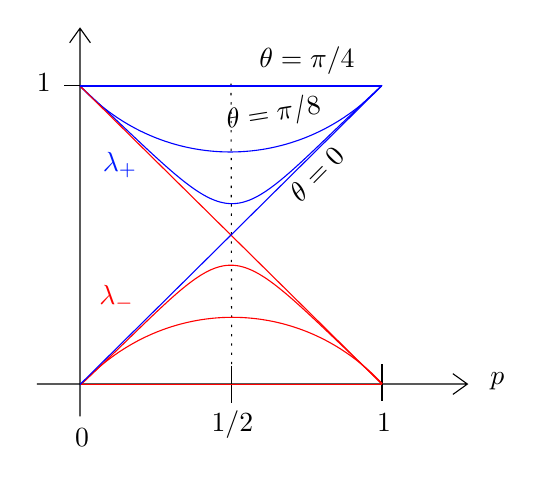
\begin{tikzpicture}[x=0.75pt,y=0.75pt,yscale=-1,xscale=1]
%uncomment if require: \path (0,300); %set diagram left start at 0, and has height of 300

%Shape: Axis 2D [id:dp7922990999691968] 
\draw  (194.43,210.47) -- (401.8,210.47)(215.16,39.04) -- (215.16,226.01) (394.8,205.47) -- (401.8,210.47) -- (394.8,215.47) (210.16,46.04) -- (215.16,39.04) -- (220.16,46.04)  ;
%Straight Lines [id:da8910069240815945] 
\draw    (360.65,200.99) -- (360.65,218.77) ;


%Straight Lines [id:da4351424487889328] 
\draw    (223.72,66.56) -- (207.26,66.56) ;


%Curve Lines [id:da30607876297229386] 
\draw [color={rgb, 255:red, 0; green, 1; blue, 255 }  ,draw opacity=1 ]   (215.16,66.89) .. controls (255,109.31) and (320.33,109.31) .. (360.65,66.55) ;


%Straight Lines [id:da747181608280644] 
\draw    (288.24,201.65) -- (288.24,219.43) ;


%Straight Lines [id:da23659034891816488] 
\draw  [dash pattern={on 0.84pt off 2.51pt}]  (287.91,65.77) -- (288.24,203.63) ;


%Curve Lines [id:da2965920062953322] 
\draw [color={rgb, 255:red, 0; green, 1; blue, 255 }  ,draw opacity=1 ]   (215.16,66.89) .. controls (297.67,143.56) and (280.33,141.46) .. (360.65,66.55) ;


%Straight Lines [id:da39006090585929143] 
\draw [color={rgb, 255:red, 255; green, 1; blue, 0 }  ,draw opacity=1 ]   (215.16,66.89) -- (360.42,210.33) ; %diag. secondaria (rossa)


%Straight Lines [id:da7695278408520292] 
\draw [color={rgb, 255:red, 255; green, 1; blue, 0 }  ,draw opacity=1 ]   (215.16,210.50) -- (360.65,210.50) ;


%Curve Lines [id:da8911454439230475] 
\draw [color={rgb, 255:red, 255; green, 1; blue, 1 }  ,draw opacity=1 ]   (360.76,210.32) .. controls (321.03,167.58) and (255.87,167.58) .. (215.65,210.67) ;


%Curve Lines [id:da5909210917925549] 
\draw [color={rgb, 255:red, 255; green, 1; blue, 1 }  ,draw opacity=1 ]   (360.76,210.32) .. controls (278.47,133.06) and (295.76,135.18) .. (215.65,210.67) ;


%Straight Lines [id:da03926817807025573] 
\draw [color={rgb, 255:red, 0; green, 1; blue, 255 }  ,draw opacity=1 ]   (215.16, 210.67) -- (360.42, 66.89) ; %diag principale (blu)


%Straight Lines [id:da42866181264009473] 
\draw [color={rgb, 255:red, 0; green, 1; blue, 255 }  ,draw opacity=1 ]   (215.16,66.89) -- (360.65,66.89) ;



% Text Node
\draw (416.28,208.92) node   {$p$};
% Text Node
\draw (234.45,105.07) node [color={rgb, 255:red, 0; green, 27; blue, 255 }  ,opacity=1 ]  {$\lambda _{+}$};
% Text Node
\draw (216.16,236.5) node   {$0$};
% Text Node
\draw (361.64,229.26) node   {$1$};
% Text Node
\draw (197.72,65.38) node   {$1$};
% Text Node
\draw (288.57,229.93) node   {$1/2$};
% Text Node
\draw (232.85,168.87) node [color={rgb, 255:red, 255; green, 0; blue, 0 }  ,opacity=1 ]  {$\lambda _{-}$};
% Text Node
\draw (324.5,54.5) node   {$\theta =\pi /4$};
% Text Node
\draw (329,109) node [rotate=-314.59]  {$\theta =0$};
% Text Node
\draw (308.5,80.5) node [rotate=-350.74]  {$\theta =\pi /8$};


\end{tikzpicture}
\caption{\footnotesize Andamento degli autovalori $\lambda_\pm$ in funzione di $p$ per alcuni valori di $\theta$ da $0$ a $\pi/4$.\label{fig:andamenti-autoval}}
\end{subfigure}%
\begin{subfigure}[t]{0.45\textwidth}
\centering


\tikzset{every picture/.style={line width=0.75pt}} %set default line width to 0.75pt        

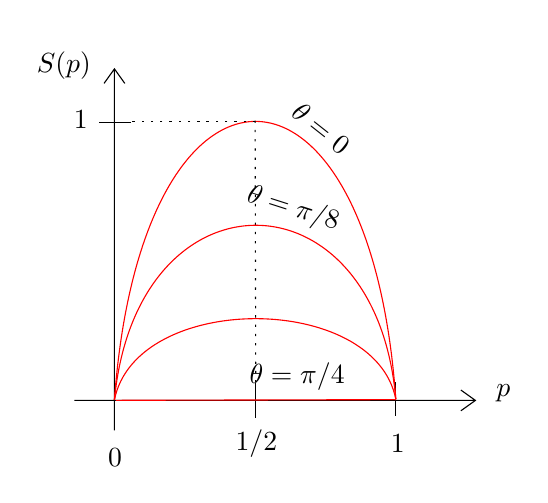
\begin{tikzpicture}[x=0.75pt,y=0.75pt,yscale=-1,xscale=1]
%uncomment if require: \path (0,300); %set diagram left start at 0, and has height of 300

%Shape: Axis 2D [id:dp5027085791119299] 
\draw  (185.02,202.37) -- (378.25,202.37)(204.34,42.64) -- (204.34,216.85) (371.25,197.37) -- (378.25,202.37) -- (371.25,207.37) (199.34,49.64) -- (204.34,42.64) -- (209.34,49.64)  ;
%Straight Lines [id:da09853418101033773] 
\draw    (339.91,193.54) -- (339.91,210.1) ;


%Straight Lines [id:da3358027007557636] 
\draw    (212.32,68.28) -- (196.98,68.28) ;


%Curve Lines [id:da3148958709948577] 
\draw [color={rgb, 255:red, 255; green, 0; blue, 0 }  ,draw opacity=1 ]   (204.34,202.13) .. controls (217.41,23.06) and (327.34,23.47) .. (339.91,201.82) ;


%Straight Lines [id:da8089499215946534] 
\draw    (272.43,194.15) -- (272.43,210.72) ;


%Straight Lines [id:da23335895135809026] 
\draw  [dash pattern={on 0.84pt off 2.51pt}]  (272.13,67.54) -- (272.43,195.99) ;


%Straight Lines [id:da42484056815365134] 
\draw  [dash pattern={on 0.84pt off 2.51pt}]  (272.13,68.03) -- (212.75,68.03) ;


%Curve Lines [id:da04941603137640582] 
\draw [color={rgb, 255:red, 255; green, 0; blue, 0 }  ,draw opacity=1 ]   (204.34,202.13) .. controls (215,89.67) and (330.33,90.33) .. (339.91,201.82) ;


%Straight Lines [id:da510763025258693] 
\draw [color={rgb, 255:red, 255; green, 0; blue, 0 }  ,draw opacity=1 ]   (340,202) -- (205,202.33) ;


%Curve Lines [id:da015065338845632326] 
\draw [color={rgb, 255:red, 255; green, 0; blue, 0 }  ,draw opacity=1 ]   (204.34,202.13) .. controls (214.75,150) and (329.75,150) .. (339.91,201.82) ;



% Text Node
\draw (391.75,199.06) node   {$p$};
% Text Node
\draw (204.65,229.73) node   {$0$};
% Text Node
\draw (340.83,222.98) node   {$1$};
% Text Node
\draw (188.09,67.17) node   {$1$};
% Text Node
\draw (272.74,222.98) node   {$1/2$};
% Text Node
\draw (292.33,190.67) node   {$\theta =\pi /4$};
% Text Node
\draw (290.5,110.17) node [rotate=-17.78]  {$\theta =\pi /8$};
% Text Node
\draw (304,71.17) node [rotate=-38.36]  {$\theta =0$};
% Text Node
\draw (180,41) node   {$S( p)$};


\end{tikzpicture}
\caption{\footnotesize Grafico dell'entropia di von Neumann per $\theta=0,\pi/4$ e valori intermedi. Nota: per $\pi/4$ l'entropia si annulla, dato che in tal caso $\ket{a}=\ket{b}$ \label{fig:entropia-von-neumann}}
\end{subfigure}%
\caption{Grafici relativi ad una mistura statistica di stati quantistici senza analogo classico (ossia non ortogonali)}
\end{figure}
\end{document}

